\documentclass{article}
\usepackage[utf8]{inputenc}
\usepackage{fullpage}
\usepackage{graphicx}
\title{Elektrotechnik}
\author{Thierry Schwaller}
\date{November 2019}
\usepackage{graphicx}

\begin{document}
	\section{Ladung C}
	Kleinstmögliche Ladungsmenge $\rightarrow$ $q_{e} = e = -1.602 * 10^{-19}C (e = Elektron / -e = Proton).$ \\
	Jede Ladung ist ein Vielfaches von $Q = N * \pm e$
	\begin{itemize}
		\item Zwei Arten von Ladungen (+ / -)
		\item Ladung ist immer quantisiert (kleine Ladungspackete)
		\item Ladung bleibt immer erhalten in einem geschlossenen System $\rightarrow$ kann nur transportiert werden
		\item Ladung ist immer an Masse gebunden
	\end{itemize}
	\section{Strom I}
	Die Bewegung von Ladungsträgern in eine bestimmte Richtung durch eine gewisse Grenze / Grenzfläche wird der elektrische Strom genannt. \\
	Elektrischer Strom ist Ladungstransport.  l
	\begin{equation}
		\textrm{Ladungsmenge Q pro Zeit t durch eine Querschnittfläche } I = \frac{\Delta Q}{\Delta t}
	\end{equation}
	\section{Stromdichte}
	Diese Formel ist nicht allgemein gültig.
	\begin{equation}
		J = \frac{I}{A} \\
	\end{equation}
	Schmelzstromdichte $\rightarrow$ Punkt wo die Temperatur in 10ms auf die Schmelztemperatur steigt.
	\section{1.Kirchhoffsche Gesetzt (Knotensatz)}
	Die Summe aller Ströme in einem Knoten mit der selben Bezugsrichtung ist immer 0. \\
	\begin{equation}
		\sum I_{n} = 0
	\end{equation}
	\section{Potential}
	\begin{equation}
		\varphi = \frac{W}{Q}
	\end{equation}
	\begin{itemize}
		\item Potential ist Energie normalisiert durch die Ladungsmenge
		\item Potentielle Energie $W = Q * \varphi$
		\item Einheit $[\frac{J}{C}] = V$
	\end{itemize}
	\begin{figure}[htbp]
	\centering
	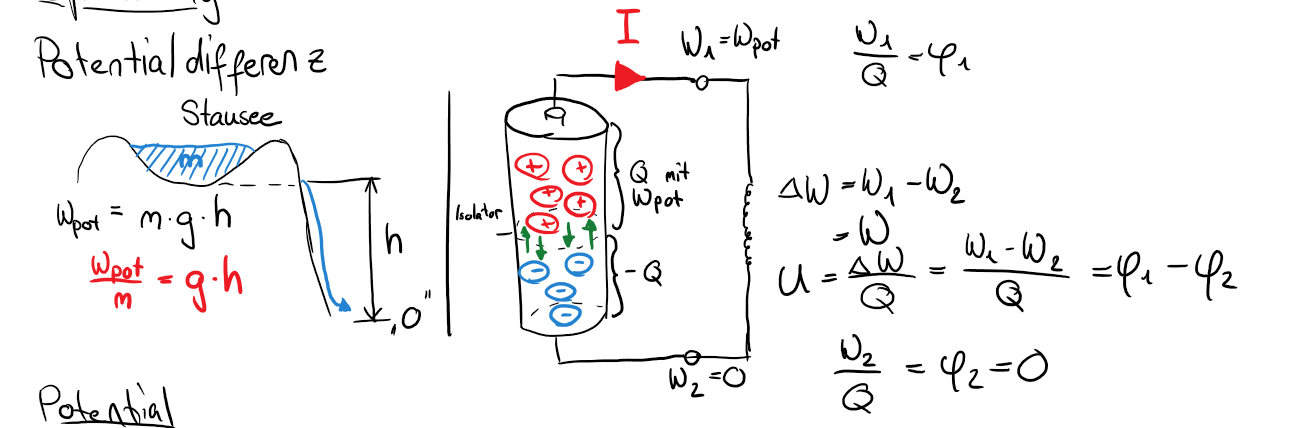
\includegraphics[width=0.5\textwidth]{Bilder/Spannung}
	\caption{Vergleich Wasser / Strom}
	\end{figure}
	\section{Spannung}
	Potentialdifferenz / Potentiell verrichtbare Arbeit. \\
	\begin{equation}
	U_{AB} = \varphi_{A} - \varphi_{B} = \frac{W_{A} - W_{B}}{Q} = \frac{\Delta W}{Q}
	\end{equation}
	Normalisierte für den Ladungstransport aufgewendete Arbeit.\\
	Für eine Sappnung braucht es lediglich eine Potentialdifferenz, es braucht nicht unbedingt einen Strom. (Spannung ist die potentielle Arbeit, welche frei würde , wenn Ladungen transportiert werden können.)
	\section{2. Kirchhoffsche Gesetz (Maschensatz)}
	Alle Teilspannungen entlang einem Umlauf innerhalb einer Masche addiert sind null.
		\begin{figure}[htbp]
		\centering
		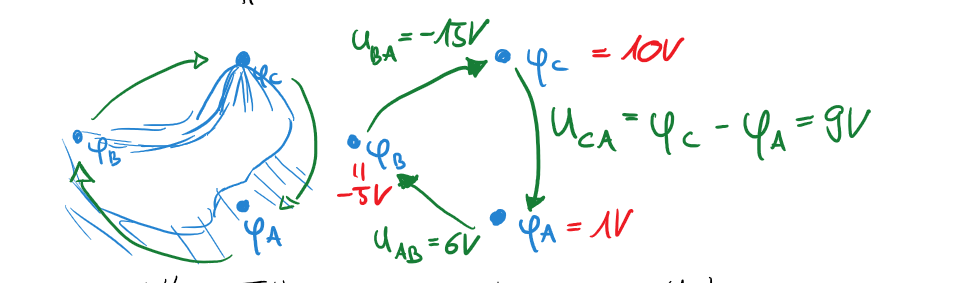
\includegraphics[width=0.7\textwidth]{Bilder/Kirchhof2}
		\caption{Maschensatz}
	\end{figure}
	\section{Leistung}
	Die Leistung ist die pro Zeiteinheit t von der Ladungsmenge Q geleistete Arbeit W. \\
	Liegt an einem elektrischen Verbraucher eine Spannung U an und wird dabei die Ladung Q transportiert, so wird Arbeit verrichtet.
	\begin{equation}
		P = \frac{W}{t} = \frac{\Delta Q * U}{\Delta t} = U * \frac{\Delta Q}{\Delta t} = U * I = [\frac{J}{s}] = Watt 
	\end{equation}
		\begin{figure}[htbp]l
		\centering
		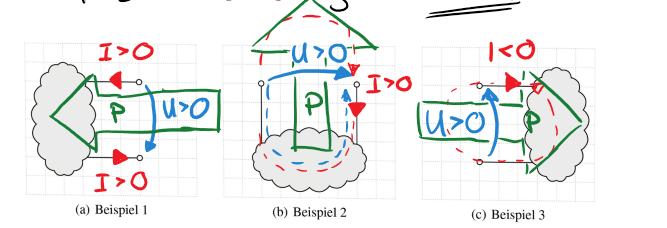
\includegraphics[width=0.7\textwidth]{Bilder/Verbraucher_Generator}
		\caption{Verbraucher oder Generator?}
	\end{figure}
	\section{Leitwert}
	Der elektrische Leitwert G eines Widerstandes ist der Proportionalitätsfaktor, welcher der Spannung über einem Widerstand dem Strom gegenüberstellt:
	\begin{equation}
		G = \frac{I}{U} \left[S \left(Siemens\right) \right] 
	\end{equation}
	Wird die Spannung (Druck auf die Ladungsträger) vergrössert, so steigt auch der Strom linear, dh der Strom durch einen Widerstand ist proportional zur Spannung darüber. 
	\section{Elektrischer Widerstand}
	Der elektrische Widerstand R ist der Kehrwert des Leitwertes und verbindet somit den Strom (Folge) mit dessen Spannung (Ursache)
	\begin{equation}
	R = \frac{U}{I} \left[\Omega \left(Ohm\right) \right] 
	\end{equation}
	\section{Elektrische Leitfähigkeit}
	Damit ein elektrischer Stromfluss möglich ist müssen freie Ladungsträger (meistens freie Elektronen / Ionen) verfügbar sein. \\
	Diese drei Faktoren bestimmen die Leitfähigkeit eines Stoffes:
	\begin{itemize}
		\item Die Anzahl freier Ladungsträger pro Volumen (freie Ladungsträgerdichte) 	$\rightarrow \textrm{In Metallen: } n_e$
		\item Die Ladung der einzelnen freien Ladungsträgern            				$\rightarrow \textrm{In Metallen: } e$
		\item Tatsächliche Beweglichkeit der freien Ladungsträgern (Elektromobilität)	$\rightarrow \textrm{In Metallen: } \mu_e$
	\end{itemize}
	\begin{equation}
		\textrm{elektrische Leitfähigkeit: } \sigma = n q \mu = \textrm{Bei Metallen: }n_e e \mu_e  \left[\frac{S}{m} \left(Siemens/Meter\right) \right]
	\end{equation}
	\subsection{Elektromobilität}
	$\tau$ ist die mittlere Stosszeit oder Zeit zwischen "Kollisionen" der Ladungsträger mit anderen Ladungsträgern und restlichen Bestandteilen des Atomgitters. \\
	$\tau$ ist umgekehrt proportional zu der Temperatur. Je höher die Temperatur desto mehr Vibration von den atomaren Bestandteilen, d.h mehr Kollisionen.
	\begin{equation}
		\textrm{Beweglichkeit: } \mu = \frac{q^\tau}{m} \left( \tau \propto \frac{1}{\sqrt{T}}\right) 
	\end{equation}
	\section{Nichtlineare Widerstände}
	Gekrümmte I-U Kennlinie $\rightarrow$ Nicht linearer Widerstand \\
	Der Widerstand R beziehungsweise der Leitwert ist die Steigung der Tangente in einem bestimmten Punkt auf der Widerstand- Leitwertkennlinie. (Die Ableitung)
	\section{Temperaturabhängigkeit}
	Metalle $\rightarrow$ Kaltleiter \\
	Ladungsträger entweder freie Elektronen oder freie Ionen. \\\\
	Wenn  $\beta \Delta T^2 \ll \alpha \Delta T$ ( $\alpha$ und $\beta$ $\rightarrow$ Temperaturkoeffizienten):
	\begin{equation}
		\Delta R \propto \Delta T \rightarrow  \Delta R = \alpha \Delta T R_T = \alpha(T - T_0)R_T
	\end{equation}
	Sonst:
	\begin{equation}
		\Delta R = (\alpha \Delta T + \beta \Delta T^2)R_T
	\end{equation}
	\section{Geschwindigkeit der freien Elektronen in metallischen Leiter}
	\begin{itemize}
		\item Driftgeschwindigkeit: mittlere Geschwindigkeit von Elektronen in Stromrichtung max. einige mm/s (von A nach B)
		\item Ausbreitungsgeschwindigkeit: "Geschwindigkeit des Signals / Impulses" 0.1 - 0.9 * $c_0$ der Lichtgeschwindigkeit
		\item Brownsche Molekular Bewegung: ungeordnete thermische Bewegung max. einige 100 km/s, im Mittel null
	\end{itemize}
	\newpage
	\section{Quellen}
	\begin{itemize}
		\item Quellenart
		\subitem Stromquelle
		\subitem Spannungsquelle
		\item Ideal / Real
		\item Abhängig / Unabhängig
		\item linear / nicht linear
	\end{itemize}
	\subsection{Ideale Quellen}
		\begin{figure}[htbp]
		\centering
		\begin{minipage}[b]{0.4 \textwidth}
			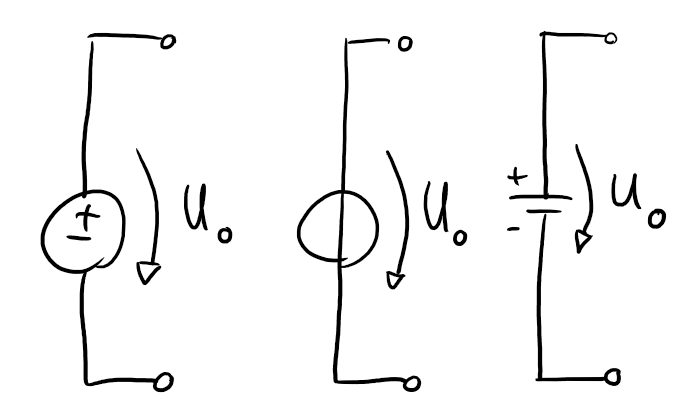
\includegraphics[width=\textwidth]{Bilder/Spannungsquelle_Ideal}
			\caption{Ideale Spannungsquelle}
		\end{minipage}
		\hfill
		\begin{minipage}[b]{0.4 \textwidth}
			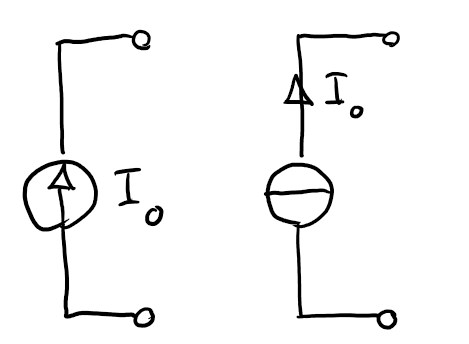
\includegraphics[width=\textwidth]{Bilder/Stromquelle_Ideal}
			\caption{Ideale Stromquelle}
		\end{minipage}
		\end{figure}
	\subsection{Reale lineare Spannungsquellen}
	Ideale Quellen gibt es in der Praxis nicht, sie werden allerdings in der Theorie gebraucht. \\
	Eine reale Spannungsquelle hat immer einen seriell geschalteten Innenwiderstand.
	\begin{figure}[htbp]l
		\centering
		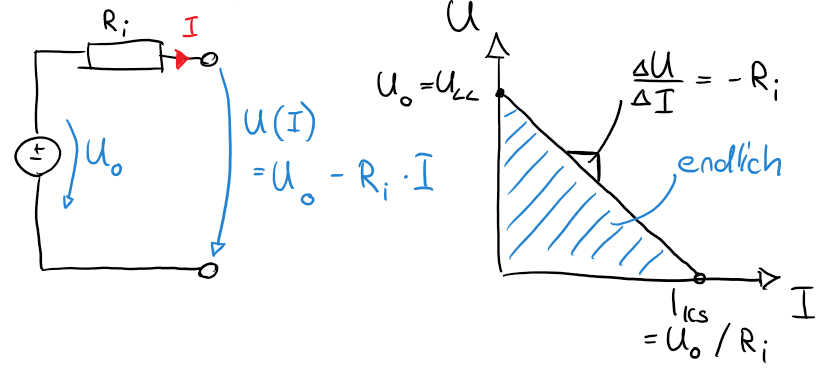
\includegraphics[width=0.7\textwidth]{Bilder/Spannungsquelle}
		\caption{Spannungsquelle}
	\end{figure} 
	\subsection{Reale lineare Stromquelle}
	\begin{figure}[htbp]
		\centering
		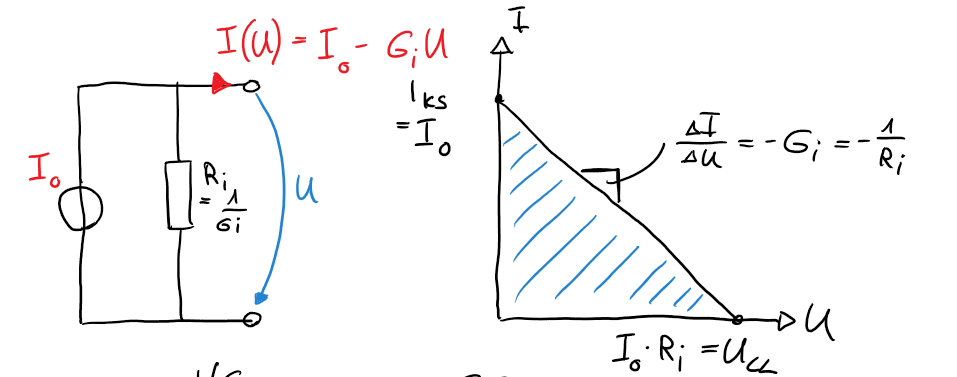
\includegraphics[width=0.5\textwidth]{Bilder/Stromquelle}
		\caption{Stromquelle}
	\end{figure}
	\subsection{Gesteuerte Quellen}
		\begin{figure}[htbp]
		\centering
		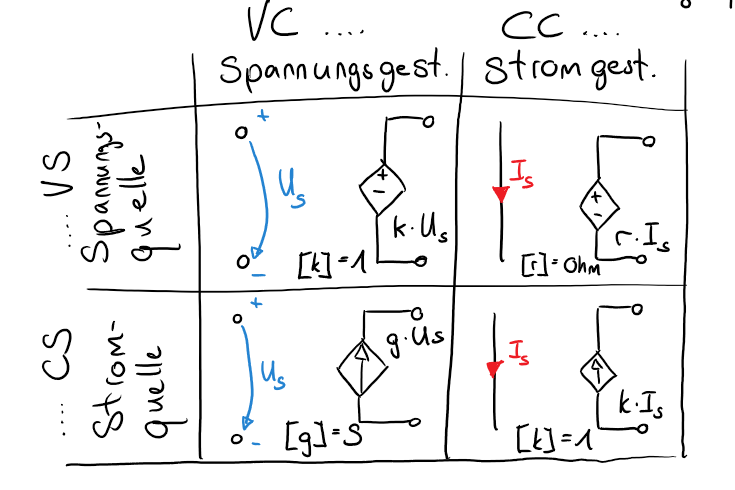
\includegraphics[width=0.6\textwidth]{Bilder/Gesteuerte_Quellen}
		\caption{Verschiedene gesteuerte Spannungs- und Stromquellen}
	\end{figure}
	\subsection{Nicht lineare Quellen}
\begin{figure}[htbp]
	\centering
	\begin{minipage}[b]{0.4 \textwidth}
		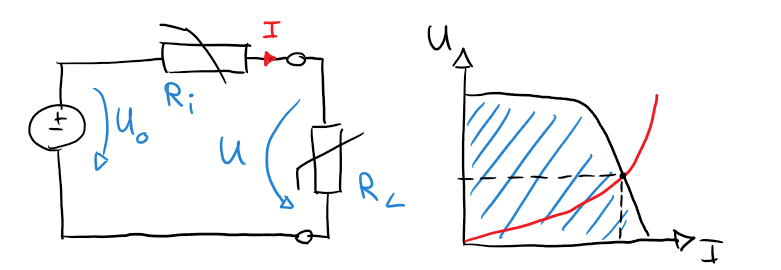
\includegraphics[width=\textwidth]{Bilder/N_L_Spannungsquelle}
		\caption{Nicht lineare Spannungsquelle}
	\end{minipage}
	\hfill
	\begin{minipage}[b]{0.4 \textwidth}
		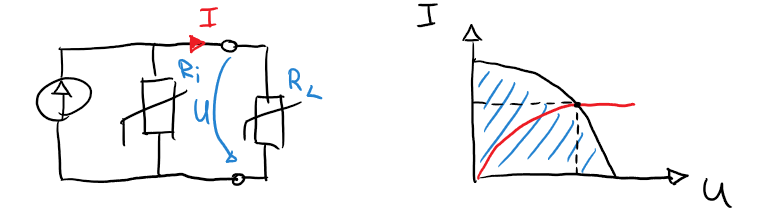
\includegraphics[width=\textwidth]{Bilder/N_L_Stromquelle}
		\caption{Nicht lineare Stromquelle}
	\end{minipage}
\end{figure}
\newpage
\section{Quellenumwandlung}
\subsection{Äquivalenz}
Die Äquivalenz ist eine bestimme Gleichheit. \\
Als Beispiel sind äquivalente Netzwerke, Netzwerke in welchen der Strom und die Spannung gleich sind (siehe Norton-Theorem).
\subsection{Thevenin - Theorem}
	Man kann jede mögliche Kombination von linearen Spannungsquellen, Stromquellen und ohmschen Widerständen bezüglich zweier Anschlussklemmen durch eine Reihenschaltung aus einer Spannungsquelle und einem ohmschen Widerstand erzeugen. \\
	\begin{figure}[htbp]
		\centering
		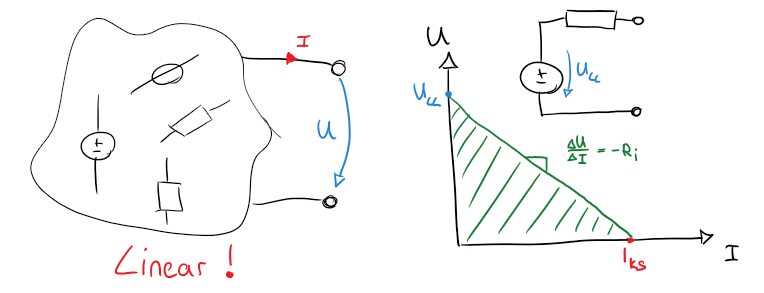
\includegraphics[width=0.6\textwidth]{Bilder/Thevenin_Theorem_Basic}
		\caption{Grundidee des Thevenin Theorems}
	\end{figure}
\subsection{Norton-Theorem}
	Jede lineare Spannungsquelle kann in eine lineare Stromquelle (Stromquelle mit parallelem Widerstand) verwandelt werden, welche bezüglich der zwei Anschlussklemmen elektrisch äquivalent ist.
\subsection{Vereinfachung von Schaltungen Thevenin/Norton}
\begin{itemize}
	\item Symetrien erkennen 
	\item Irrelevante Elemente eliminieren
	\item Gesteuerte Quellen ausschalten
	\item Von eigener Grösse abhängige Quellen in Widerstände umwandeln
	\item Superpositionsprinzip (16.5) 
	\item Reziprozität 
\end{itemize}
\subsection{Superpositionsprinzip}
Das Superpositionsprinzip ermöglicht das Berechnen von Schaltungen mit mehr als einer unabhängigen Quelle. Dieses Prinzip gilt nur in linearen Systemen. \\
Es dürfen alle unabhängigen Quellen einzeln in der Schaltung angeschaut werden (Spannungsquellen $\rightarrow$ kurzgeschlossen und Stromquellen $\rightarrow$ Unterbrüche) jedoch müssen danach alle einzelnen Werte kombiniert werden.
\begin{figure}[htbp]
	\centering
	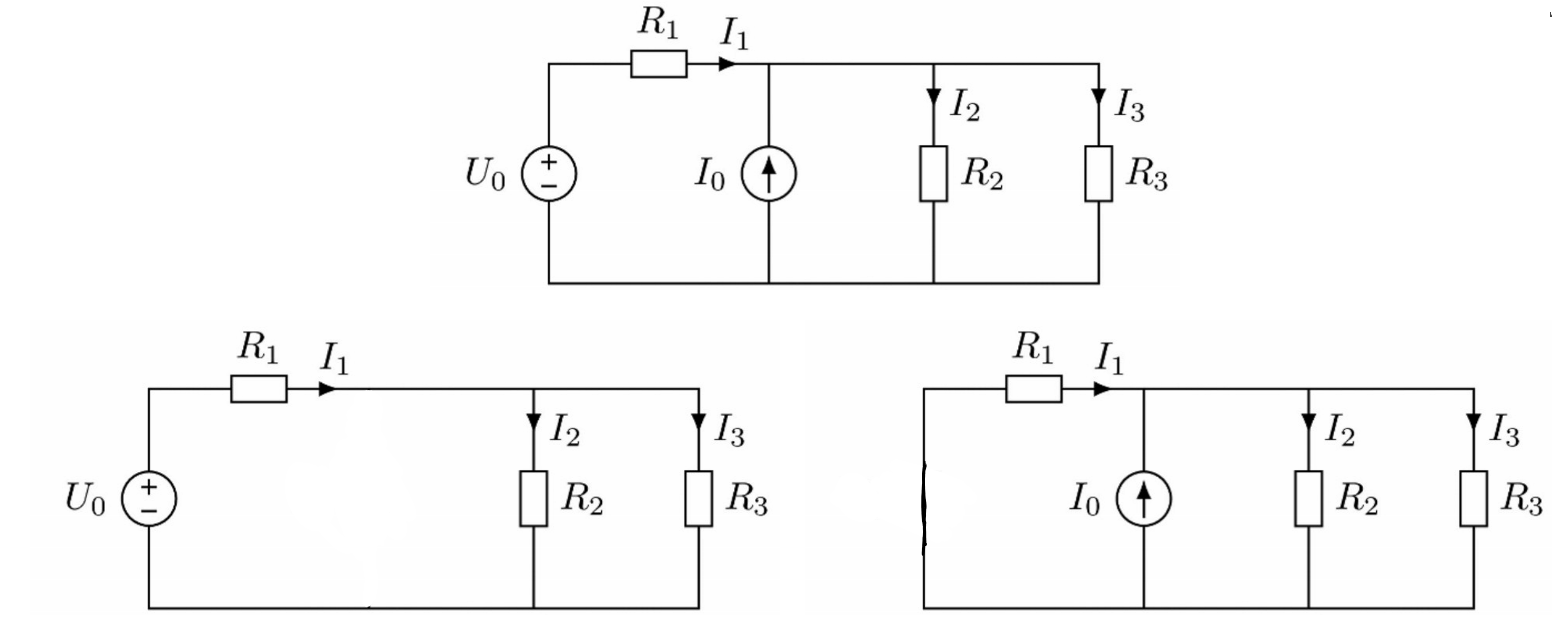
\includegraphics[width=0.6\textwidth]{Bilder/Superpositionsprinzip}
	\caption{Superpositionsprinzip mit 2 Quellen}
\end{figure}
\section{Elementare Schaltungen}
\subsection{Spannungsteiler}
Werden mehrere Widerstände in Serie geschalteten teilt sich die Gesamtspannung in Teilspannungen über den verschiedenen Widerständen auf. Dies nennt man ein Spannungsteiler
\subsubsection{Unbelastete Spannungsteiler}
Besteht aus einer Masche, in welcher überall der gleiche Strom fliest. \\
Das Verhältnis jeder Teilspannung $U_n$ ist zur Gesamtspannung $U_0$ gleich wie der zugehörige Widerstand zum Gesamtwiderstand. 
\begin{equation}
	\frac{U_1}{U_2} = \frac{R_1}{R_2} \textrm{ und } \frac{U_2}{U_0} = \frac{R2}{R1 + R2}
\end{equation}
\begin{figure}[htbp]
	\centering
	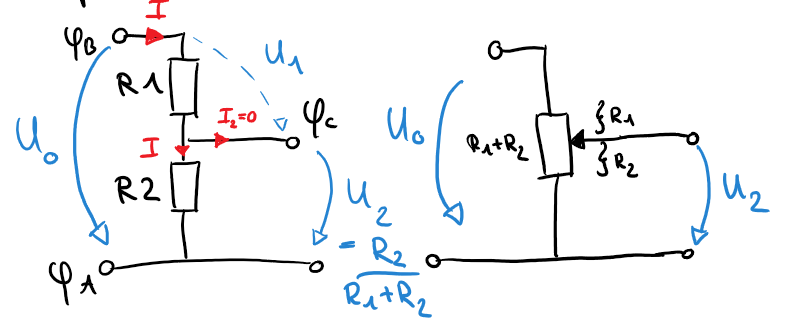
\includegraphics[width=0.5\textwidth]{Bilder/Spannungsteiler_unb}
	\caption{Unbelastete Spannungsquelle}
\end{figure}
\subsubsection{Belasteter Spannungsteiler}
\begin{figure}[htbp]
	\centering
	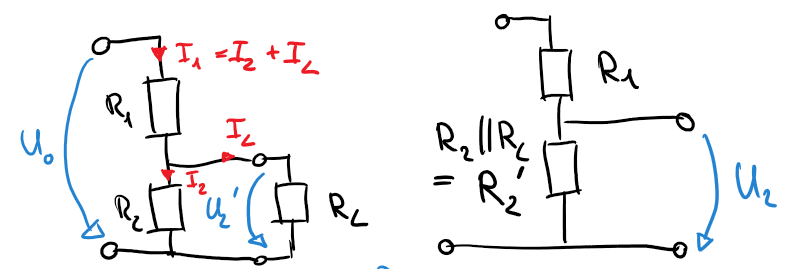
\includegraphics[width=0.5\textwidth]{Bilder/BelasteterSpannungsteiler}
	\caption{Belasteter Spannungsteiler}
\end{figure}
\begin{equation}
	R'_2 = R_2 || R_L = \frac{R_2 R_L}{R_2 + R_L}
\end{equation}
Mit dieser Formel hat man danach wieder einen unbelasteten Spannungsteiler und kann mit der Formel 13 rechnen ($R_2 = R'_2$).
\subsection{Stromteiler}
\subsubsection{Unbelasteter Stromteiler}
Besteht aus einer Parallelschaltung in welcher überall die selbe Spannung herrscht. \\
Der Strom teilt sich proportional zum Leitwert (oder umgekehrt proportional zu dem Widerstand) auf. 
\begin{equation}
	I_1 = \frac{U}{R_1} \textrm{ und } I_2 = \frac{U}{R_2}
\end{equation} 
Die Ströme teilen sich so auf:
\begin{equation}
\frac{I_1}{I_2} = \frac{U / R_1}{U / R_2} = \frac{R_2}{R_1} = \frac{G_1}{G_2}
\end{equation}
Und der Gesamtstrom:
\begin{equation}
\frac{I_2}{I_0} = \frac{R_{tot}}{R_2} 
\end{equation}
\begin{figure}[htbp]
	\centering
	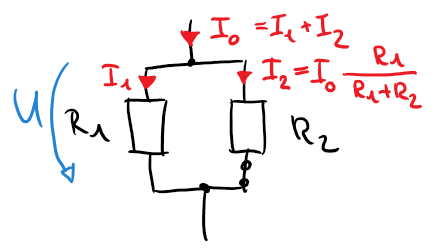
\includegraphics[width=0.35\textwidth]{Bilder/Unb_Stromteiler}
	\caption{Unbelasteter Stromteiler}
\end{figure}
\subsubsection{Belasteter Stromteiler}
\begin{figure}[htbp]
	\centering
	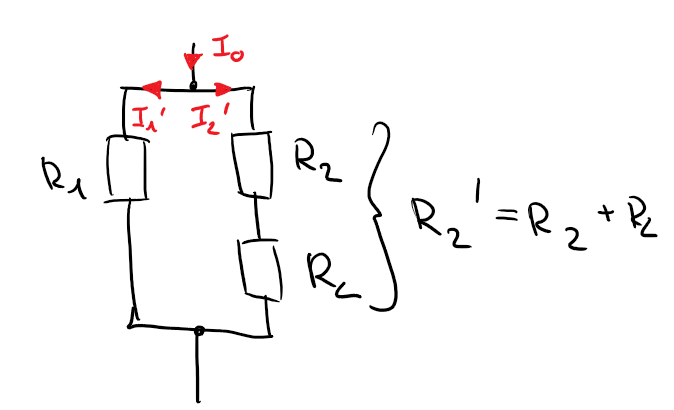
\includegraphics[width=0.4\textwidth]{Bilder/BelasteterStromteiler}
	\caption{Belasteter Stromteiler}
\end{figure}
\begin{equation}
	R'_2 = R_2 + R_L
\end{equation}
Mit dieser Formel hat man danach wieder einen unbelasteten Stromteiler und kann mit den Formeln 15/16/17 rechnen.
\subsection{Brückenschaltung}
Kombination aus Spannungs- und Stromteiler
\begin{figure}[htbp]
	\centering
	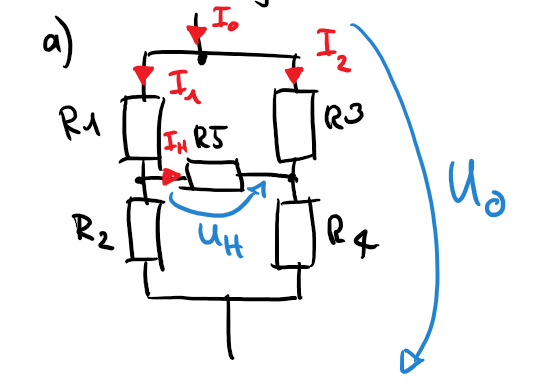
\includegraphics[width=0.4\textwidth]{Bilder/Bruckenschaltung}
	\caption{Brückenschaltung}
\end{figure}
\begin{itemize}
	\item Stern-Dreieck-Umwandlung 
	\subitem Zum Beispiel R1/R2/R5 können in eine Dreieckschaltung umgewandelt werden. Danach besteht die Schaltung aus einem dreifachen Stromteiler, mit zwei Serienschaltungen. 
	\item Dreieck-Stern-Umwandlung
	\subitem R2,R4 und R5 können in einen Stern umgewandelt werden. Danach besteht die Schaltung aus einem Spannungsteiler mit einem Stromteiler als einer der Widerstände.
	\item Potentialberechnung von zwei realen Quellen
	\subitem Oftmals ist es hilfreich beide Spannungsteiler als reale Quellen zu betrachten welche  gegeneinander mit dem Brückenwiderstand R5 belastet werden
\end{itemize}
\section{Reziprozität / Kirchhoffsche Umkehrungssatz}
Der Kirchhoffsche Umkehrungssatz gilt nur für Netzwerke mit einer Quelle. (Superpositionsprinzip auch) \\
Bei der Anwendung des Reziprozitätstheorems muss jeweils auf die Polarität der Quellen und gemessenen Grössen geachtet werden.
Es gibt 2 Arten von Reziprozität: \\
\begin{itemize}
	\item Spannungsquelle
	\subitem Der Strom I resultiert auch im Zweig der Quelle wenn diese dort ausgeschaltet und an der vorherigen Messstelle eingebaut wird.
	\begin{figure}[htbp]
		\centering
		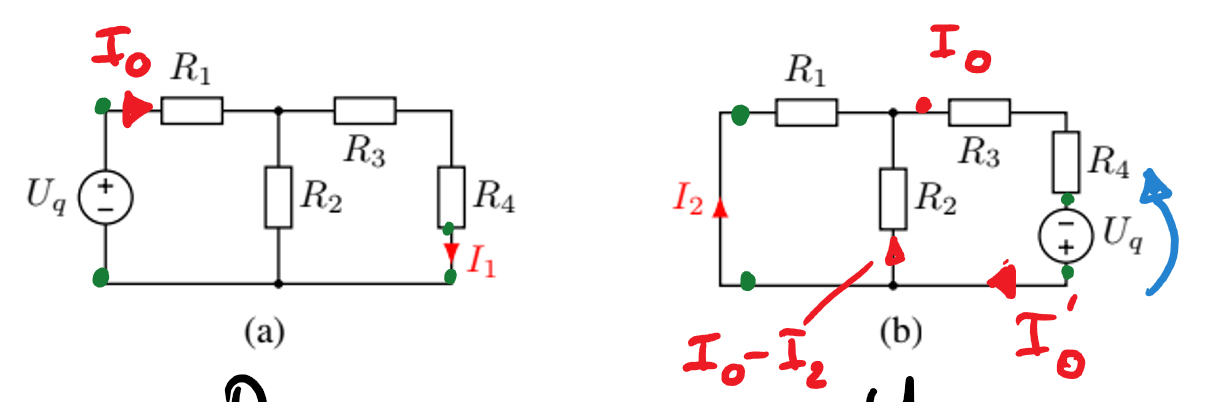
\includegraphics[width=0.6\textwidth]{Bilder/Reziprozitat_Spannungsquelle}
	\end{figure}
	\item Stromquelle
	\subitem Die Spannung U resultiert auch zwischen den Anschlüssen der Quelle, wenn diese dort ausgeschalten und zwischen den vorherigen beiden Messknoten angehängt wird.
	\begin{figure}[htbp]
		\centering
		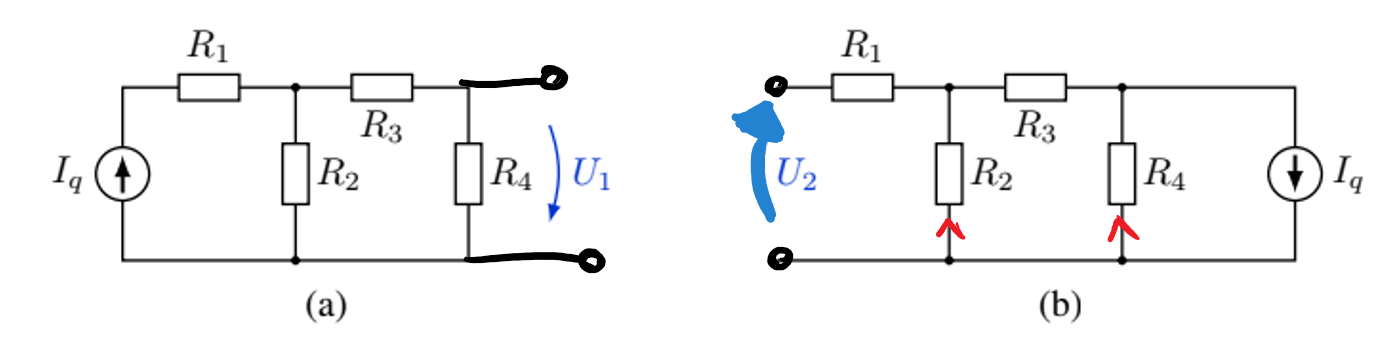
\includegraphics[width=0.6\textwidth]{Bilder/Reziprozitat_Stromquelle}
	\end{figure}
\end{itemize}
\section{Leistung}
\subsection{Allgemein}
\begin{equation}
	\eta = \frac{\Delta W_{ab}}{\Delta W_{zu}}
\end{equation}
In der Elektrotechnik erfolgt die Abgabe der Nutzenergie gleichzeitig mit der Energieaufnahme. "Arbeit $\Delta W =$ Leistung P über eine gewisse Dauer $\Delta t$" daher kann der Wirkungsgrad auch als Verhältnis der abgegebenen Nutzleistung $P_{ab}$ zur Gesamtleistung ausgedrückt werden:
\begin{equation}
\eta = \frac{P_{ab}}{P{zu}}
\end{equation}
\subsection{Leistungsanpassung}
Es gibt zwei verschiedene Ziele für die Leistungsanpassung:
\begin{itemize}
	\item Möglichst Verlustarm (Energietechnik)
	\item Möglichst hohe Leistung aus Quelle beziehen (Nachrichtentechnik)
\end{itemize}
\newpage
\section{Netzwerk-Analyse}
Wird benötigt um ein lineares Netzwerk fast immer genau gleich zu analysieren.

\subsection{Graphen Theorie}
\subsubsection{Basics}
Ein Graph besteht aus Knoten und Zweigen. Die Knoten werden durch die Zweige untereinander verbunden. \\
\begin{center}
    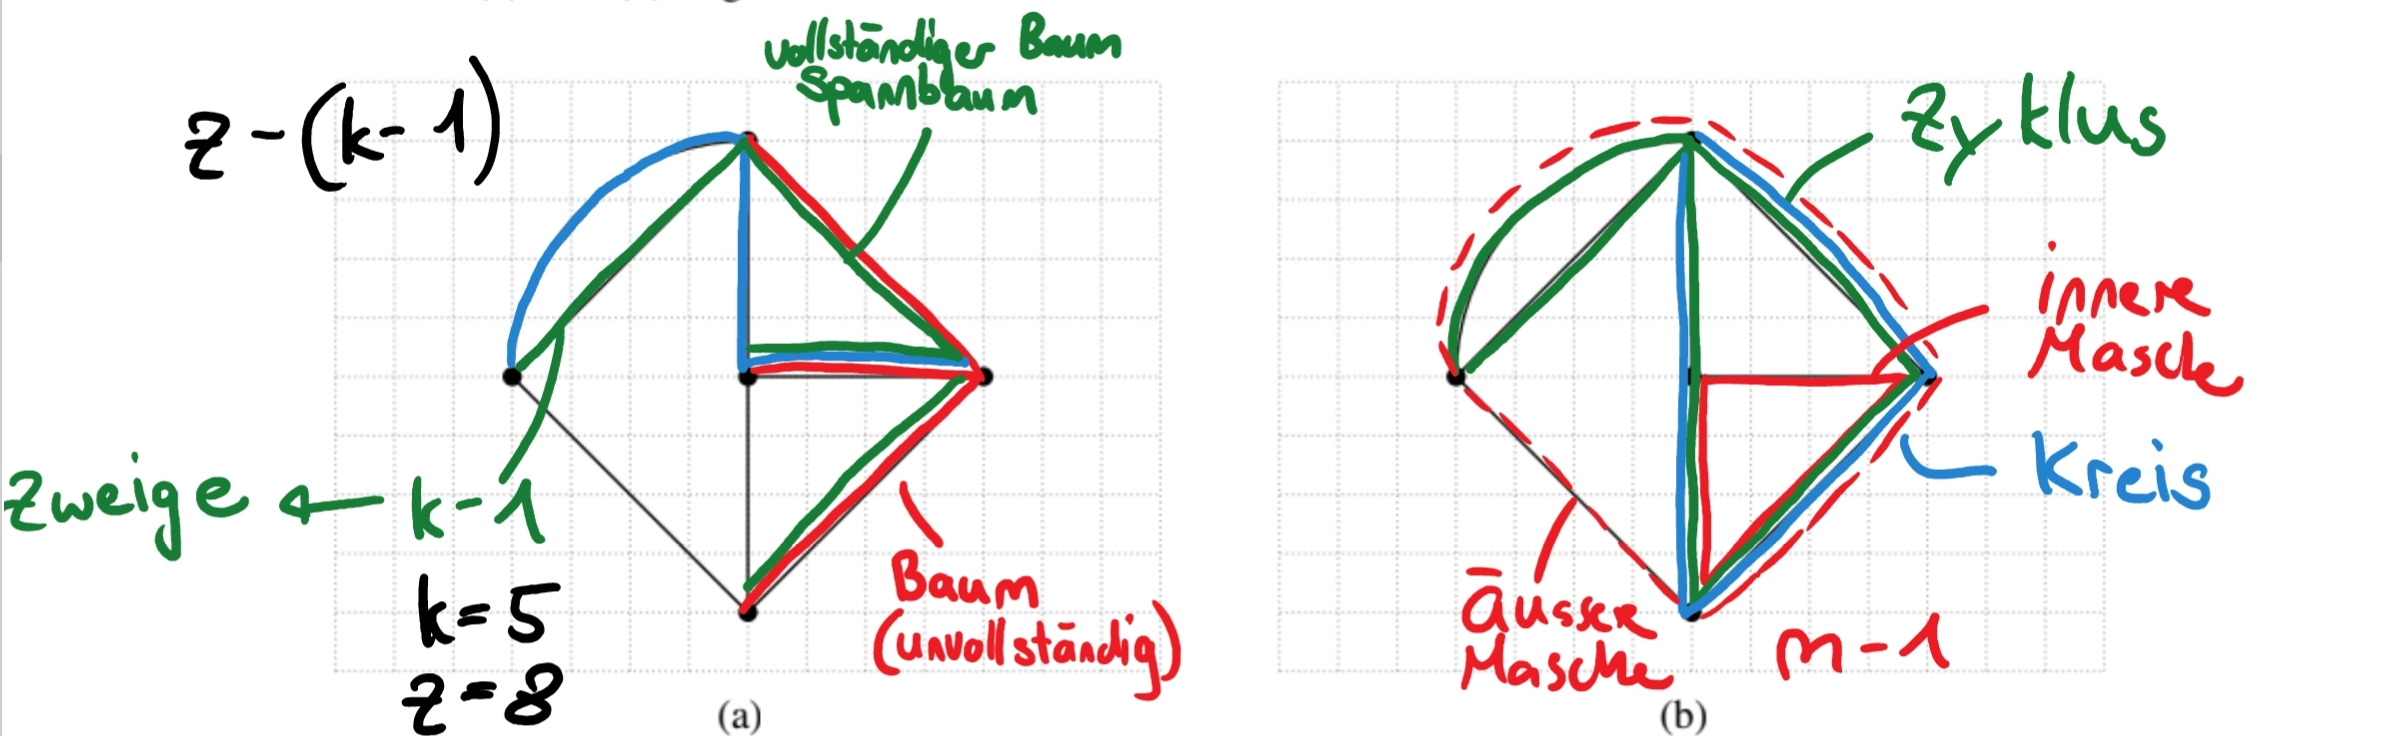
\includegraphics[width=0.7\textwidth]{Bilder/Basis_Graph_2.jpg}
\end{center}

\begin{itemize}
    \item Weg: Eine Zusammenhängende Reihe aus unterschiedlichen Kanten (keine Kante doppelt)
    \item Baum: Nicht geschlossener Weg
    \item Spannbaum: Ein Baum welcher alle Knoten des Graphne mit einander verbinden
    \item Zyklus: Weg mit gleichem Start- und Endknoten
    \item Kreis: Zyklus, welcher alle Knoten nur eimal enthält.
    \item Masche: Eine Masche ist ein Kreis welcher innterhalb oder ausserhalb keine Zweige enthält.
\end{itemize}
\subsubsection{Planare und nicht planare Graphen}
\subsection{Zweigstromanalyse}
\subsubsection{Basics}
Bevor die Zweigstrom-Analyse durchgeführt wird müssen üblicherweise diese Schritte schon gemacht worden sein.
\begin{itemize}
    \item Bereiche welche nur aus Widerständen bestehen werden durch einen einzelnen Widerstand ersetzt.
    \item ??? Bei Stromquellen wird ihr Innenwiderstand sowie alle zusätzlichen zur Quelle parallelgeschalteten Widerstände durch einen Widerstand ersetzt.
    \item Bei Spannungsquellen werden der Innenwiderstand und alle zusätzlichen in Serie geschalteten Widerstände dirch einen einzigen äquivalenten Widerstand zusammengefasst.
\end{itemize}
Nach dieser Vereinfachung hat das Netzwerk nun k Knoten und z Zweige von welchen v ideale Quellen sind.\\ \\
Unbekannte: 2z - v \\
Variablen: z
\subsubsection{Funktion / Beispiel}
Ablauf: \\
\begin{enumerate}
    \item Vereinfachung des Schaltung und bestimmung der Knoten
    \item Für jeden Zweig die Stromrichtung definieren und die k - 1 Knotengleichungen aufstellen (Kirchhoff 1)
    \item Relevante Maschen identifizieren und Umlaufrichtungen definieren.z - k + 1 Maschengleichungen (Kirchhoff 2) aufstellen.
    \item n - 1 Zweiggleichungen (Beziehung zwischen Zweigstrom und Zweigspannung) formulieren
    \item Knoten- und Maschengleichungen mit Zweiggleichungen kombinieren.
    \item Gleichungen in Matrix-Form bringen / lösen.
\end{enumerate}
\subsection{Maschenstromverfahren}
Unbekannte: m - 1 - i (i = Anzahl idealer Stromquellen) \\

Beispiel Maschenstromverfahren
\begin{enumerate}
    \item Knoten bestimmen und Spannbaum erstellen (Spannbaum möglichst nicht durch eine ideale Stronquelle)
    \item m - 1 Maschenströme bestimmen und Richtung angeben (immer die gleiche Richtung wählen)
    \item 3 Matrizen aufstellen
    \begin{equation}
        R * j = u
    \end{equation}
    \subitem \textbf{Vektor j} (m-1 * 1) beinhaltet alle Unbekannten
    \subitem \textbf{Widerstandsmatrix R} (m-1 * m-1)
    \subitem \textbf{Quellenmatrix} (m-1 * 1) 
    \item Gesteuerte Quellen hinzufügen (Sektion 3.2)
\end{enumerate}
\subsubsection{Spezialfall: Ideale Stromquelle}
Der Spannbaum darf nicht durch eine ideale Stromquelle hindurchführen. Falls dies allerdings nicht zu verhindert ist muss die Schaltung zu einer äquivalenten Schaltung umgezeichnet werden. \\

\begin{center}
    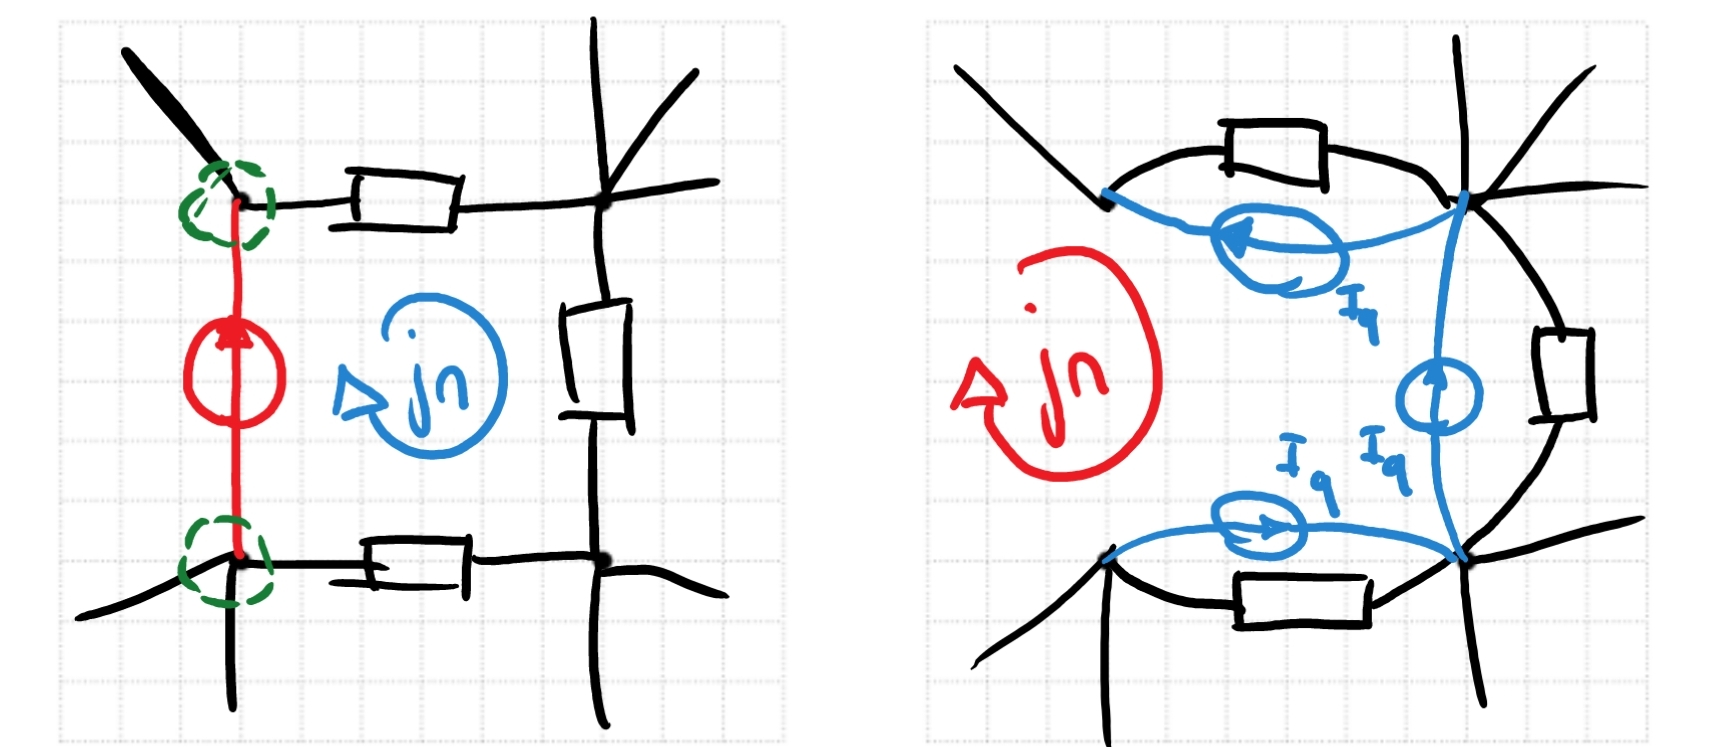
\includegraphics[width=0.7\textwidth]{Bilder/Stromquellen.jpg}
\end{center}
\subsubsection{Beispiel mit gesteuerte Quellen}

Beispiel Maschenstromverfahren mit gesteuerter Stromquelle befindet sich auf OneNote

\subsection{Knotenpotentialmethode}
Unbekannte: k - v - 1 (v $\rightarrow$ ideale Spannungsquellen) \\
\begin{enumerate}
    \item Knoten und Referenzknoten (am besten gut vernetzt und an vielen Quellen angeschlossen) bestimmen / Aufwand berechnen (k - 1 - v Gleichungen)
    \item Matrix aufstellen
    \begin{equation}
        G * u = i
    \end{equation}
    \subitem \textbf{Unbekannten Matrix u}: (k-v-1 * 1) 
    \subitem \textbf{Kehrwert-Matrix G}: (k-v-1 * k-v-1)
    \subitem \textbf{Quellen-Matrix i}: (k-v-1 * 1)
    \end{enumerate}
    Beispiel Knotenpotentialmethode befindet sich auf OneNOte
    
    \subsection{Ideale Spannungsquelle zwischen 2 Knoten}
    \begin{center}
        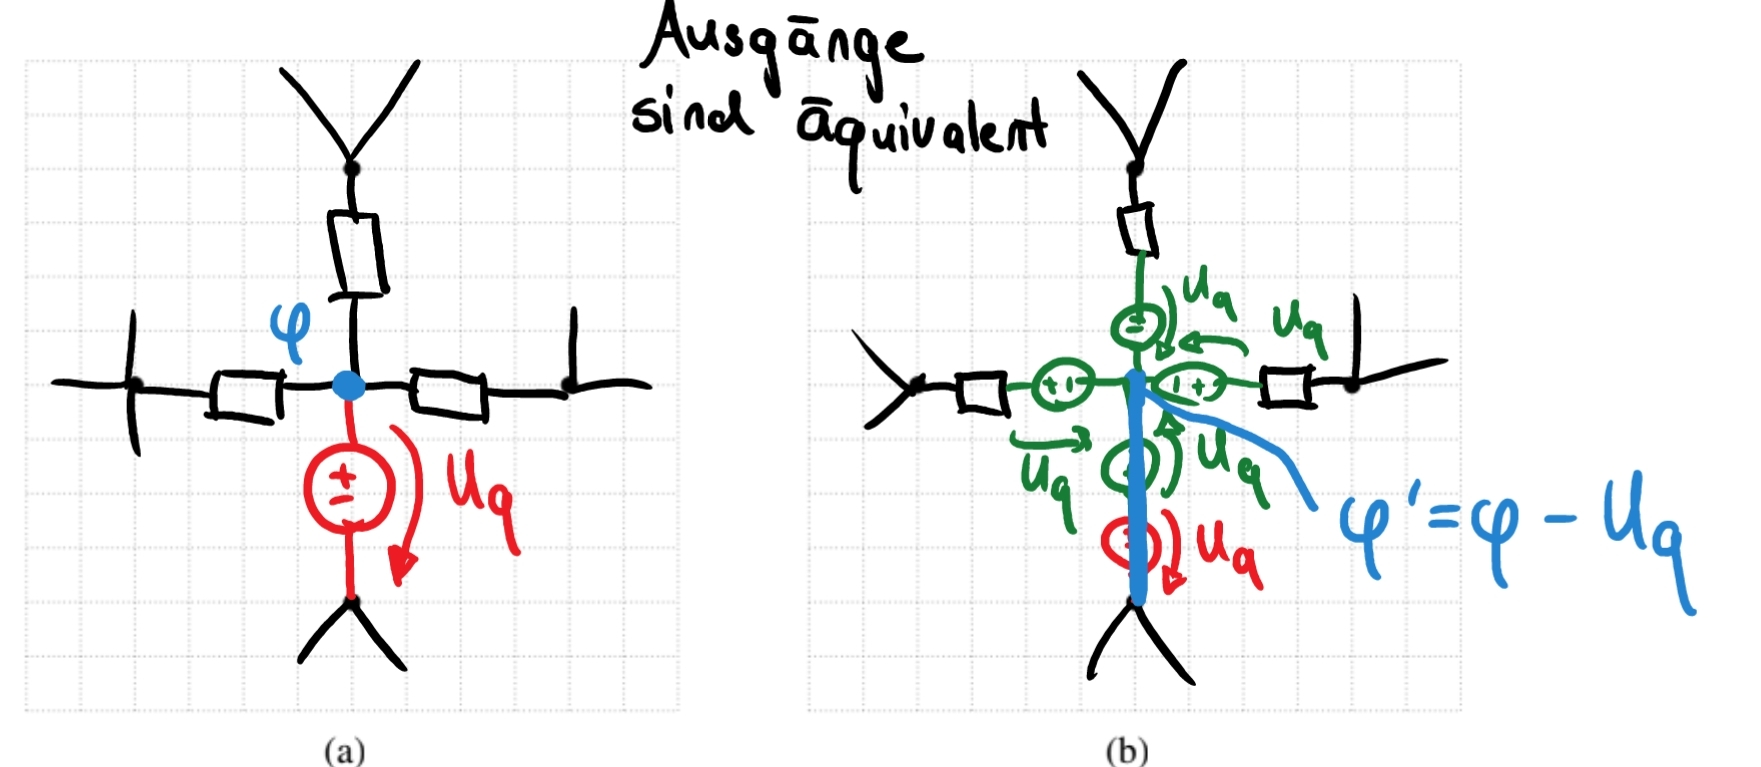
\includegraphics[width=0.7\textwidth]{Bilder/Spannungsquellen.jpg}
    \end{center}
    \subsection{Modifizierte Knotenpotentialmethode}
    Die modifizierte Knotenpotentialmethode ist aufwendiger als die KPM und MSM Methoden allerdings muss das Schema vor Beginn nicht angepasst werden, dies führt dazu das diese Methode in allen modernen Netzwerkanalyse-Tools gebraucht wird.
    \subsubsection{Anwendung}
    Der Aufwand für die MNA (Modified Nodal Analysis) beträgt: k - 1+ v (Ideale Spannungsquellen) + $i_s$ (Anzahl gesuchter Ströme). \\
    
    \subsubsection{Gesteuerte Quellen}
    \subsubsection{Elementstempel}
    \newpage
    \section{Leistungsanpassung in nicht linearen Systemen}
    \section{Strömungsfelder}
    \subsection{Grundbegriffe}
    \begin{itemize}
        \item \textbf{Feld}
        \subitem Ansammlung von mathematischen Objekten mit einer örtlichen Komponenten (Koordinatensystem)(zum Beispiel Ansammlung von Skalaren)
        \item \textbf{Skalarfeld}
        \subitem Ansammlung von Skalaren in einem Feld
        \item\textbf{Vektorfeld}
        \subitem Ansammlung von Vektoren in einem Feld.
    \end{itemize}
    Vektorenfelder können verschiedene Eigenschaften besitzen: 
    \begin{itemize}
        \item \textbf{Homogen vs. Inhomogen}
        \subitem Ein homogenes Feld hat in jedem Punkt des Feldes derselbe Vektor. Die Feldlinien verlaufen parallel.
        \item \textbf{Eben vs. Uneben}
        \subitem Ein Vektorfeld ist homogen wenn eine Ebene gewählt werden kann welche zu allen Vektoren parallel liegt.
    \end{itemize}
    \begin{center}
        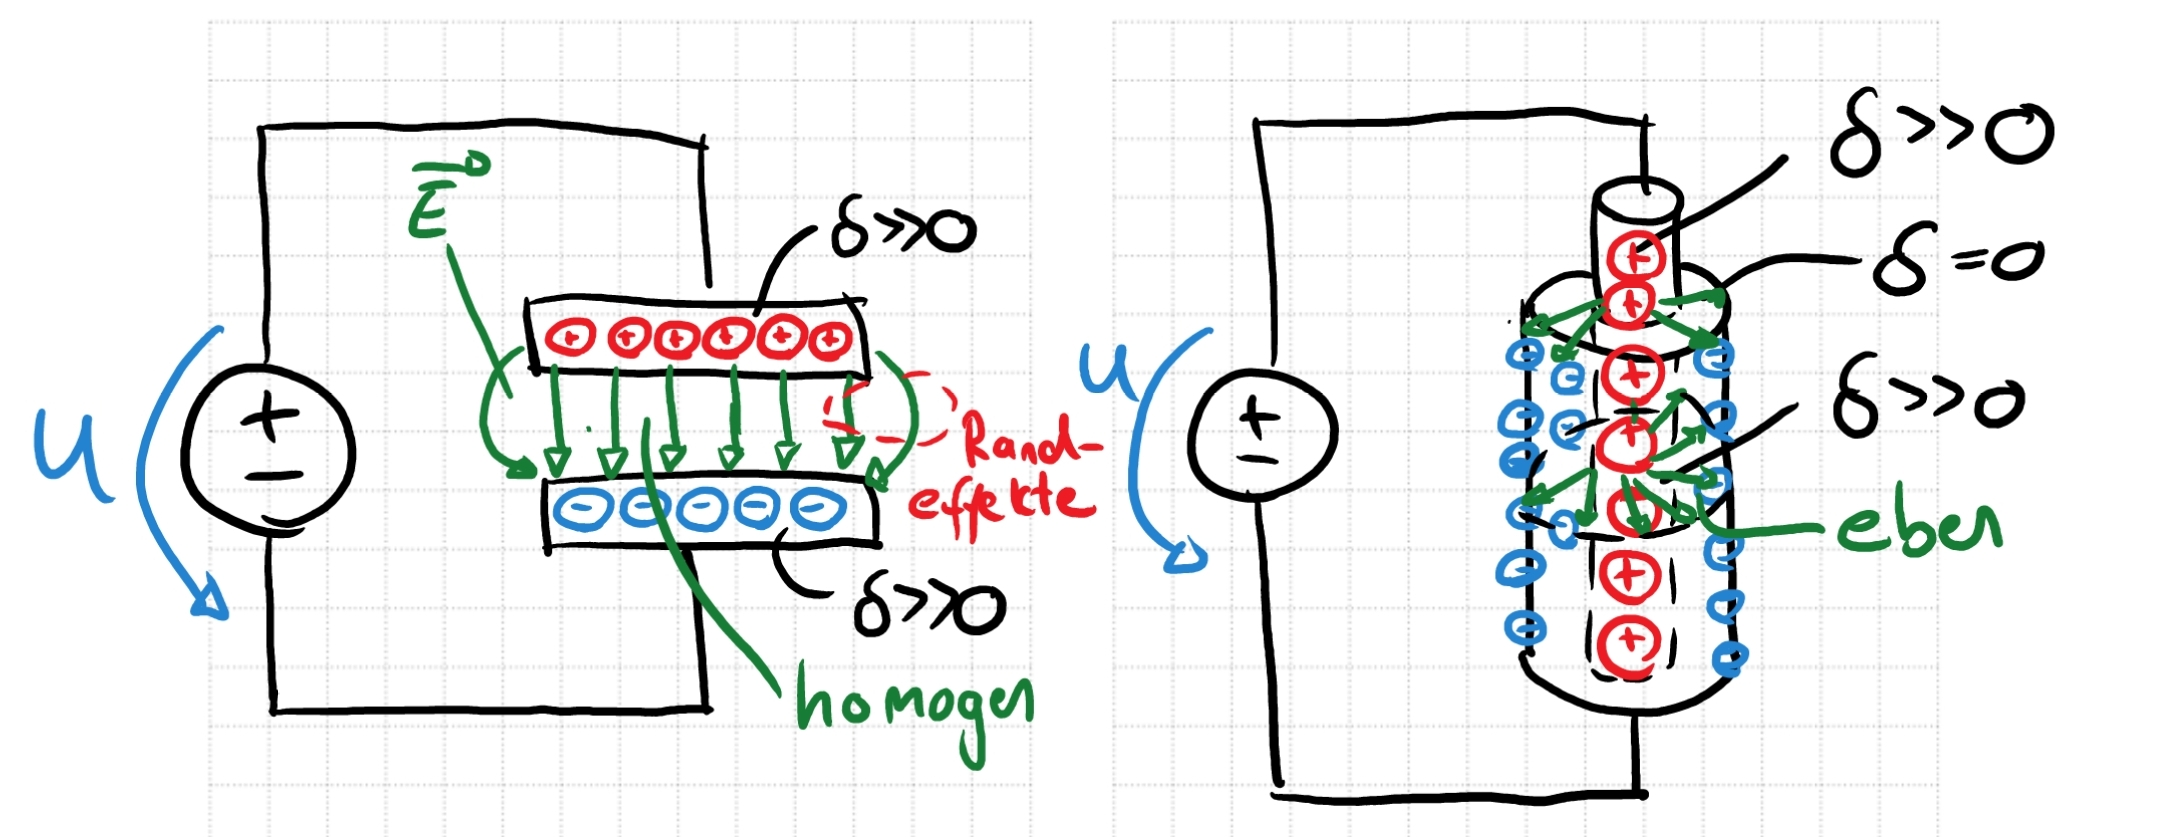
\includegraphics[width=0.7\textwidth]{SmartSelect_20191212-184142_OneNote.jpg}
    \end{center}
    Es werden hauptsächlich zwei verschiedene Darstellungsarten gebraucht um ein Strömungsfeld darzustellen. Es gibt keine bessere oder schlehtere Darstellungsart jede hat ihre eigenen Vor- und Nachteile:
    \begin{itemize}
        \item \textbf{Vektordarstellung}
        \subitem In dieser Darstellung werden Vektoren in ein Koordinatensystem gezeichnet und die Länger der Vektoren bestimmt die Intensität des Feldes am Ursprung. Da die Vektoren eine bestimmte Länge haben kann es passieren dass sie sich zu fest überlagern und die Darstellung unübersichtlhc wird.
        \item \textbf{Feldlinien}
        \subitem Feldlinien sind gerichtete Linien. Die Intensität des Feldes an einem bestimmten Punkt wird durch den Abstand der verschiedenen Feldlinien dargestellt.
    \end{itemize}
    Man unterscheidet zwischen zwei verschiedenen Feldarten die Wirbelfelder und die Quellenfelder. Bei den Wirbelfeldern bilden die Feldlinien ein geschlossenes System (sogennante Wirble) im Gegensatz zu den Quellenfelder.
    \begin{center}
        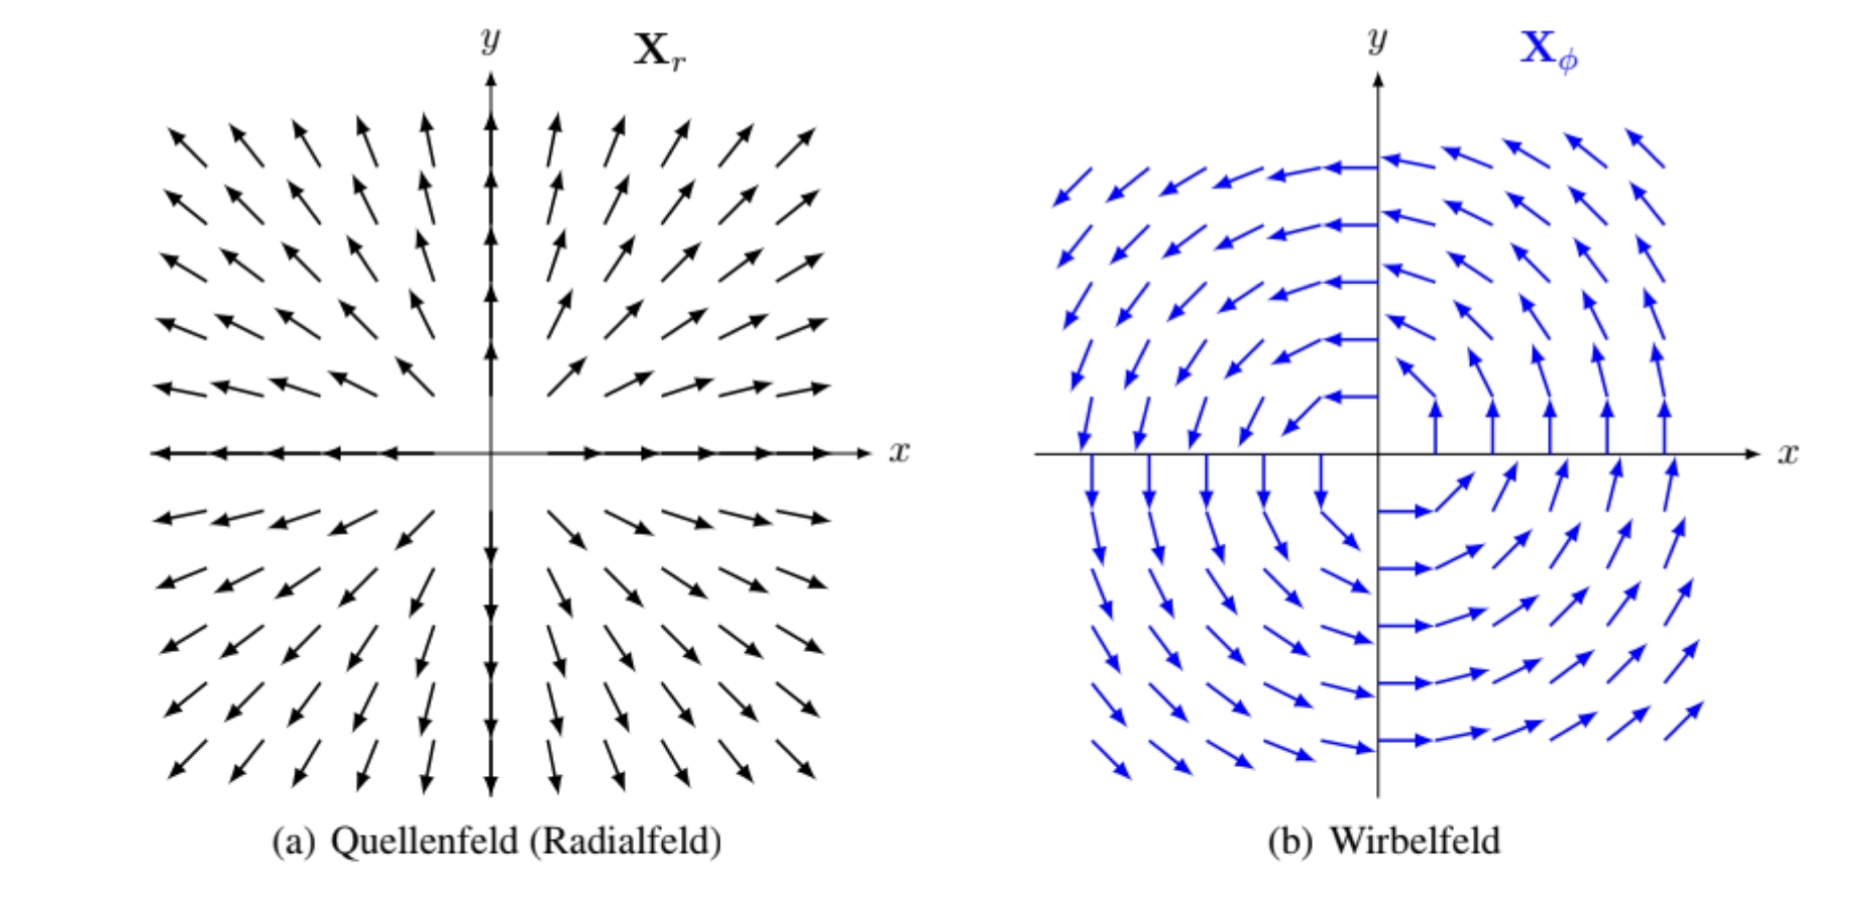
\includegraphics[width=0.7\textwidth]{SmartSelect_20191212-181204_OneNote.jpg}
    \end{center}
    Diese zwei Strömungsfelder ergeben laut dem Helmholz-Theorem das tätsächliche Strömungfeld (zum Vergleich: Superposition)
    \begin{equation}
        \textrm{Helmholz-Theorem: } X = X_r + X_O
    \end{equation}
    Dies ergibt dann:
    \begin{center}
        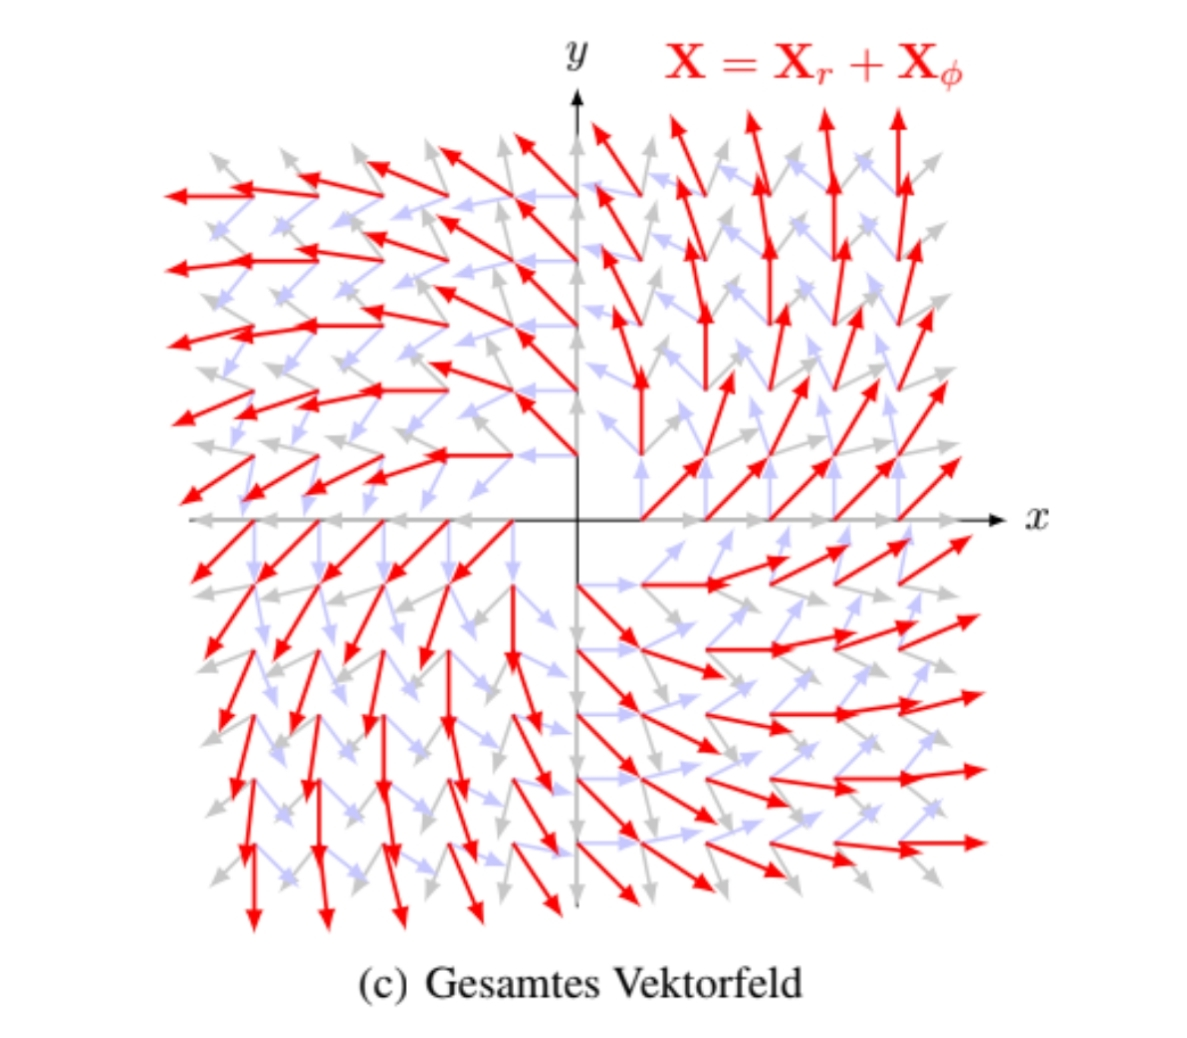
\includegraphics[width=0.5\textwidth]{SmartSelect_20191212-182306_OneNote.jpg}
    \end{center}
    \subsection{Allgemein Basics}
    Das elektrische Strömungsfeld beschreibt der Transport von elektischer Ladung. Da Ladung nur in leitenden Materialien existiert existiert ein elektrisches Strömungsfeld auch nur in leitenden Materialien. \\
    Die Stärke und die Richtung des Ladungstransportes kann ortsabhängig sein. Man spricht von einer stationären Strömung wenn die Strömungsgeschwindigkeit sowie der durchflossene Leiterquerschnitt konstant sind.
    \subsection{Die Strömungsdichte im Strömungsfeld}
    \subsubsection{Homogenes Strömungsfeld}
    
\end{document}
